\documentclass[varwidth]{standalone}
\usepackage{tikz}

\usetikzlibrary{math}
% \usetikzlibrary{external}
% \tikzexternalize


\begin{document}


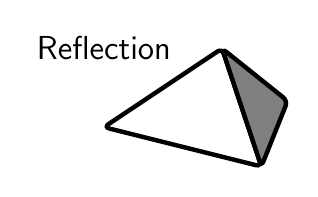
\begin{tikzpicture}[scale=0.5]
  \tikzmath{%
    \px = 1; \py = 2; \qx = 4; \qy = 4; \rx = 5; \ry = 1;
    \cx = (\px + \qx + \rx)/3; \cy = (\py + \qy + \ry)/3;
    \reflpx = 2*\cx - \px; \reflpy = 2*\cy - \py;
  } 
  
  \draw[ultra thick, rounded corners=2pt] (\px,\py)--(\qx,\qy)--(\rx,\ry)--cycle;
  \draw[ultra thick, rounded corners=2pt, fill=gray] (\reflpx,\reflpy)--(\qx,\qy)--(\rx,\ry)--cycle;

  \node at (1, 4){\large \sf Reflection};
\end{tikzpicture}
% Same line
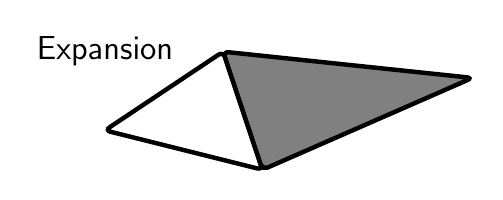
\begin{tikzpicture}[scale=0.5]
  \tikzmath{%
    \px = 1; \py = 2; \qx = 4; \qy = 4; \rx = 5; \ry = 1;
    \cx = (\px + \qx + \rx)/3; \cy = (\py + \qy + \ry)/3;
    \bb = 3;
    \exppx = (1+\bb)*\cx - \bb*\px; \exppy = (1+\bb)*\cy - \bb*\py;
  } 
  
  \draw[ultra thick, rounded corners=2pt] (\px,\py)--(\qx,\qy)--(\rx,\ry)--cycle;
  \draw[ultra thick, rounded corners=2pt, fill=gray] (\exppx,\exppy)--(\qx,\qy)--(\rx,\ry)--cycle;

    \node at (1, 4){\large \sf Expansion};
\end{tikzpicture}

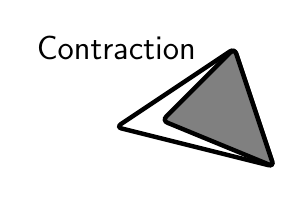
\begin{tikzpicture}[scale=0.5]
  \tikzmath{%
    \px = 1; \py = 2; \qx = 4; \qy = 4; \rx = 5; \ry = 1;
    \cx = (\px + \qx + \rx)/3; \cy = (\py + \qy + \ry)/3;
    \g = 1/2;
    \contrpx = (1 - \g)*\cx + \g*\px; \contrpy = (1 - \g)*\cy + \g*\py; 
  } 
  
  \draw[ultra thick, rounded corners=2pt] (\px,\py)--(\qx,\qy)--(\rx,\ry)--cycle;
  \draw[ultra thick, rounded corners=2pt, fill=gray] (\contrpx,\contrpy)--(\qx,\qy)--(\rx,\ry)--cycle;

  \node at (1, 4){\large \sf Contraction};
\end{tikzpicture}
% Same line
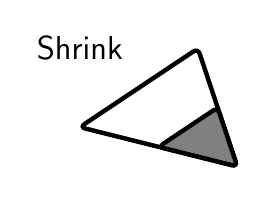
\begin{tikzpicture}[scale=0.5]
  \tikzmath{%
    \px = 1; \py = 2; \qx = 4; \qy = 4; \rx = 5; \ry = 1;
    \cx = (\px + \qx + \rx)/3; \cy = (\py + \qy + \ry)/3;
    \d = 1/2;
    \shrinkpx = \rx + \d*(\px - \rx); \shrinkpy = \ry + \d*(\py - \ry);
    \shrinkqx = \rx + \d*(\qx - \rx); \shrinkqy = \ry + \d*(\qy - \ry);
  }
  
  \draw[ultra thick, rounded corners=2pt] (\px,\py)--(\qx,\qy)--(\rx,\ry)--cycle;
  \draw[ultra thick, rounded corners=2pt, fill=gray] (\shrinkpx,\shrinkpy)--(\shrinkqx,\shrinkqy)--(\rx,\ry)--cycle;

  \node at (1, 4){\large \sf Shrink};
\end{tikzpicture}



\end{document}

